% -*- coding: utf-8 -*-
\section{Basis Sets in Quantum Chemistry}\label{basis_set_sec}

\begin{flushright}
  {\small
  ``{\em There are probably as many basis set defined for polyatomic
         calculations \\  as quantum chemists.}''
  
  -Attila Szabo and Neil S. Ostlund
  }
\end{flushright}

\noindent The choice of a basis set has a fundamental importance in quantum
chemical calculations, as it directly influences both the accuracy of the
results and the computational cost. Basis sets provide a finite, predefined
collection of functions in which the molecular orbitals are expanded, and the
mathematical properties of these functions determine how well they can describe
features such as electron density, polarisation and correlation effects
\cite{szabo, jensen2013introduction}. A well-chosen basis set ensures that the
quantum mechanical approximation has an accurate outcome while maintaining
computational efficiency.

A key concept in basis set construction is the so-called ``zeta'' quality,
which refers to the number of basis functions used per atomic orbital. A
single-$\zeta$ (SZ) basis set uses one function per orbital and offers only a
minimal description of the electronic structure. A double-$\zeta$ (DZ) basis set
adds a second, independently optimised function per orbital, thereby increasing
variational flexibility and allowing the orbitals to contract or expand
depending on the chemical environment. Higher levels, such as triple-$\zeta$ (TZ)
and quadruple-$\zeta$ (QZ) sets, include three and four functions per orbital,
respectively, and systematically improve the representation of the molecular
wavefunction~\cite{Dunning1989, Weigend2005}. These higher-$\zeta$ basis sets
enable a better treatment of electron correlation by providing more accurate
orbital shapes and greater angular momentum mixing.  However, each increase in
$\zeta$ quality incurs a substantial computational overhead, and thus the
trade-off between accuracy and cost must be carefully considered.

It is also crucial to emphasise that basis set quality is not solely determined
by the number of radial functions ($\zeta$ level), but also by the angular
flexibility of the set. This means that functions with higher angular momentum
($p$, $d$, $f$, etc.) must be included to accurately describe anisotropic
electron distributions and polarisation effects. For example, the unperturbed
hydrogen atom requires only a single $1s$ orbital for its exact wavefunction.
However, when exposed to an external electric field, the spherical symmetry is
broken, and the electron density becomes displaced. To describe this polarised
density, $p$-type functions must be incorporated. Similarly, for second-row
elements like carbon, nitrogen, and oxygen, the inclusion of $d$-type
polarisation functions significantly improves accuracy~\cite{Jensen2001},
particularly in chemical environments where the electron cloud is perturbed by
the natural non-uniform distribution of electron density. These polarisation
functions are essential for reproducing subtle features of the electron density
in molecular systems.

\subsubsection{Slater-Type Basis Sets}

When solving the Schrödinger Equation for the hydrogen atom, the analytical
solutions yield orbitals that exhibit the correct cusp behavior at the nucleus
and an exponential decay at large distances. These features are naturally
captured by Slater-Type Orbitals (\glspl{STO}), which are typically expressed as:

\begin{align}
  \chi_{\mathrm{STO}}(\mathbf{r}) = N r^{n-1} e^{-\zeta r},
\end{align}

\noindent where $N$ is a normalisation constant, $n$ is the principal quantum
number, and $\zeta$ is an orbital exponent controlling the radial decay. The
\glspl{STO} provide a physical realism, especially an accurate representation of
electron density near and far away the nucleus.

\newpage
However, the evaluation of multicenter integrals with \glspl{STO} is
mathematically and computataionally cumbersome because the exponential form
complicates the solution of two-electron integrals, that problem is the
motivation for the development of different approximations, such as the
Gaussian-Type Orbitals (\gls{GTO}) and plane-wave basis sets.

\subsubsection{Gaussian-type Basis Sets}

To overcome the challenges associated with \glspl{STO}, Gaussian-Type Orbitals
(\glspl{GTO}), first introduced by Boys~\cite{boys1950}, quickly gained
popularity and have become the standard in many quantum chemistry applications.
A typical Gaussian function is written as:

\begin{align}
  \chi_{\mathrm{GTO}}(\mathbf{r}) = N x^l y^m z^n e^{-\alpha r^2},
\end{align}

\noindent with $N$ as the normalisation constant, $l$, $m$, and $n$ as the
angular momentum components, and $\alpha$ setting the width of the Gaussian.

Thanks to the Gaussian Product Theorem~\cite{Besal2011}, the product of two
Gaussians yields another Gaussian centered along the interatomic axis, which
allows four-center integrals to reduce systematically into a hierarchy of
simpler integrals. This property permits an efficient evaluation of many of the
integrals encountered in \gls{HF} and post-HF methods.

Because a single Gaussian function does not reproduce the sharp nuclear cusp or
the correct asymptotic decay observed with \glspl{STO}, a linear combination of
Gaussian functions is employed to approximate a single \gls{STO}. For example,
the STO-3G basis set uses three primitive Gaussian functions to emulate the
radial behavior of a Slater orbital. Although this contracted Gaussian approach
sacrifices some accuracy in reproducing fine details of the electron density
(particularly near and far from the nucleus), it represents a well-balanced
compromise between computational efficiency and accuracy.

\newpage
\subsubsection{Plane-Wave Basis Sets}

In a different approach, plane wave basis sets are widely used in the study of
periodic and extended systems, such as those found in solid-state physics. A
plane wave basis function is given by:

\begin{align}
  \chi_{\mathrm{PW}}(\mathbf{r}) = \frac1{\sqrt{V}} e^{i \mathbf{k} \cdot \mathbf{r}},
\end{align}

\noindent where $V$ is the normalised volume of the unit cell and $\mathbf{k}$
is the reciprocal lattice vector.

Plane waves are especially advantageous to describe delocalized electronic
states under periodic boundary conditions. Their systematic convergence is
controlled by the kinetic energy cutoff, however, a large number of basis
functions are required to accurately describe localized features like core
electrons.  Therefore, although plane-wave basis sets are well suited for
periodic systems, they are less efficient when applied to isolated molecules.

\subsection{Selecting a Basis Set}

In summary, the choice between \glspl{STO}, \gls{GTO}, or plane waves involves
a trade-off between physical accuracy and computational efficiency:

\begin{itemize}
  \item \textbf{STOs}, high physical accuracy but are computationally
    demanding, particularly for multicenter integrals.
  \item \textbf{GTOs}, provide greater computational efficiency, though at the
    cost of reduced accuracy in representing localised features.
  \item \textbf{Plane waves}, well suited for periodic systems but perform
    poorly in describing localised phenomena.
\end{itemize}

\newpage
Many quantum chemistry packages provide a wide range of basis sets. For
example, \ams~\cite{ams2025} offers several \gls{STO} basis sets, while
programs such as \gseize~\cite{g16} and \textsc{Orca}~\cite{ORCA} include an
extensive selection of \gls{GTO} basis sets. In contrast, plane-wave basis sets
are commonly used in codes like \textsc{Quantum
Espresso}~\cite{quantum_espresso} and \textsc{Vasp}~\cite{Kresse1996CMS}, which
are specifically designed for periodic systems.

% Many quantum chemistry codes offer a variety of basis sets. For instance, the
% \ams~\cite{ams2025} programs provides multiple \gls{STO} basis sets, while programs
% such as \linebreak[4]\mbox{\gseize~\cite{g16}} and \textsc{Orca}~\cite{ORCA} offer an extensive
% selection of \gls{GTO} basis sets. In contrast, plane-wave methods are typically
% employed in codes like \textsc{Quantum Espresso}~\cite{quantum_espresso} and
% \textsc{Vasp}~\cite{Kresse1996CMS}, which are tailored to periodic systems.

Majority of the quantum chemistry codes can also read basis sets provided by
the user, the
\href{https://www.basissetexchange.org/}{\textsc{BasisSetExchange} database}~\cite{Pritchard2019}
lists a wide range of basis sets.

However, it is important to note that since the mathematical properties of the
\glspl{STO}, \glspl{GTO} and plane waves are different, the software designed
to work with one type of basis set may not be able to handle the other types.

\begin{quote}
  \textit{... the choice of a basis set is not nearly the black art,\\
  \hspace*{0.57\textwidth}\makebox[0pt][r] however,\\
  \hspace*{0.61\textwidth}\makebox[0pt][r] it may first appear.}
  \begin{flushright}
    \citet{szabo}
  \end{flushright}
\end{quote}

The choice of basis set depends not only on its functional type ---whether
\glspl{STO}, \glspl{GTO}, or plane waves--- but also on the number and nature of
functions included. Higher $\zeta$ levels offer greater variational flexibility,
while polarisation functions are essential for describing anisotropic effects.
Ultimately, basis set selection reflects a trade-off between accuracy and
computational cost.

\newpage
\vspace{5cm}
For visual comparisons, Figure \ref{bs_gto_sto} illustrates the wavefunction
and the radial distribution for the hydrogen 1s orbital using different basis
sets.

\begin{figure}[h]
  \centering

  \begin{subfigure}[b]{0.65\textwidth}
    \centering
    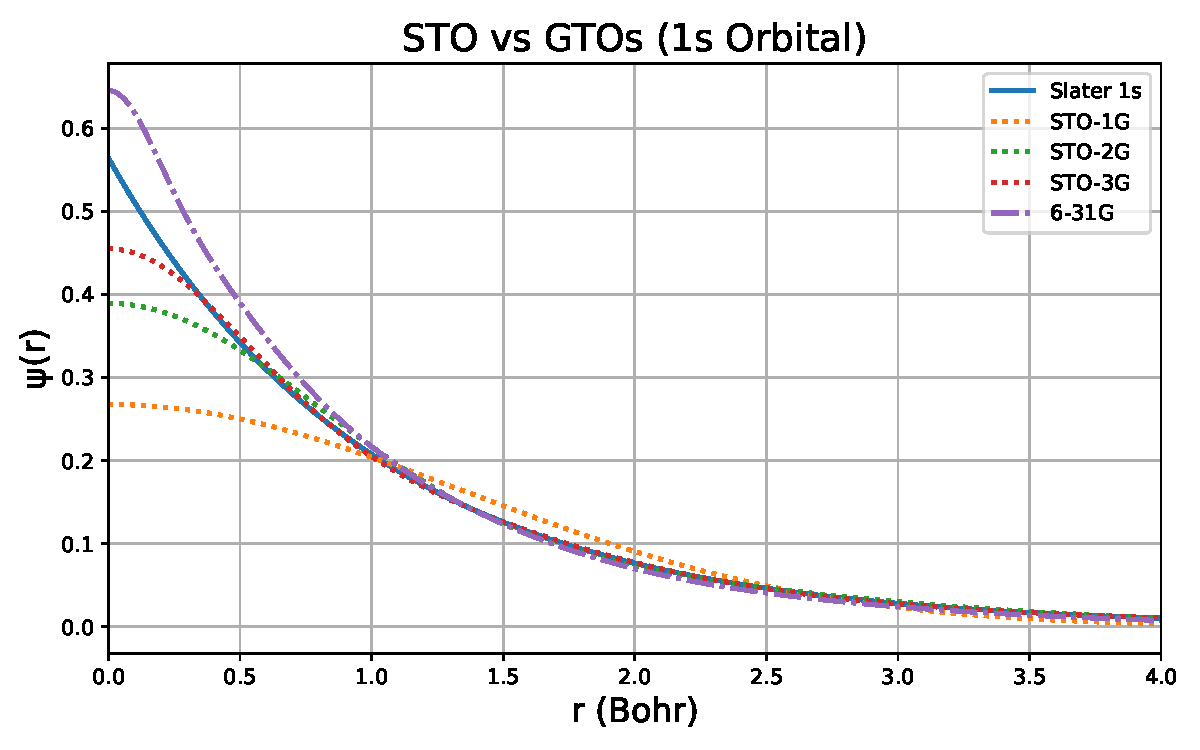
\includegraphics[width=\textwidth]{plt/gauss_slater_wavef.pdf}
    \caption{Comparison of a Slater function with Gaussian functions.
             Least squares fit of a $1s$ Slater function $\zeta$ = 1.0.}
  \end{subfigure}

  \begin{subfigure}[b]{0.65\textwidth}
    \centering
    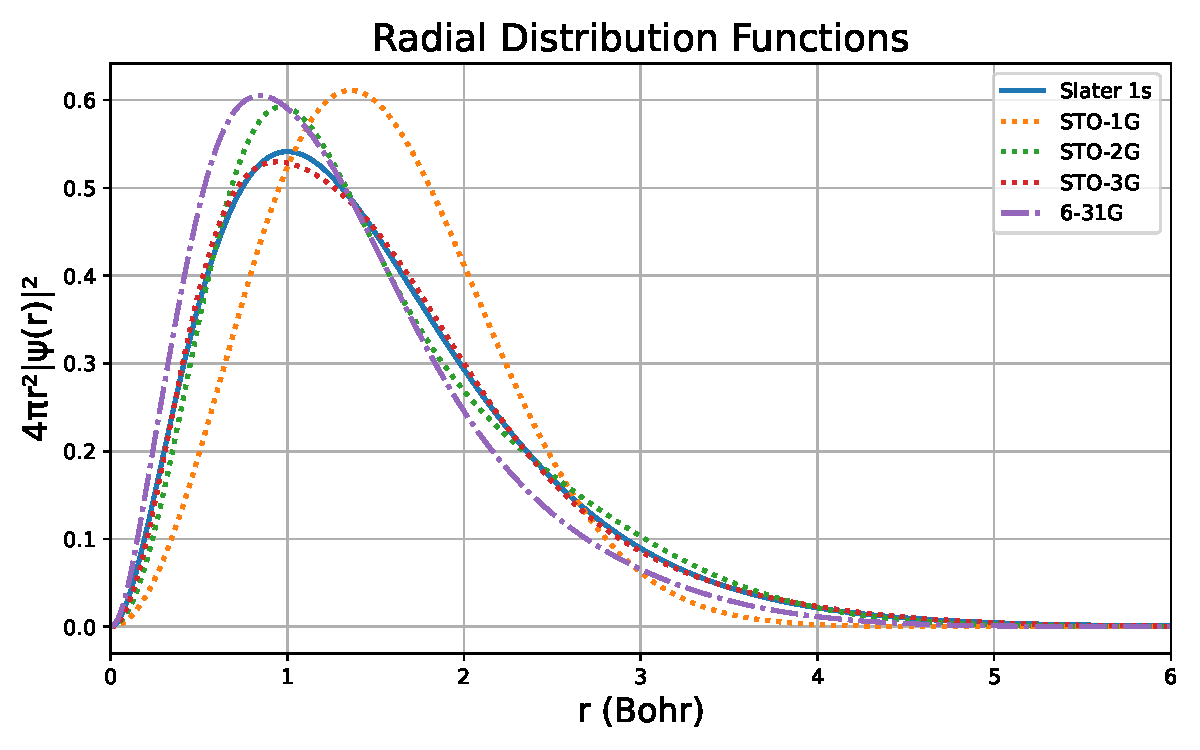
\includegraphics[width=\textwidth]{plt/gauss_slater_radial.pdf}
    \caption{Comprasion of the corresponding radial distribution functions.}
  \end{subfigure}

  \caption{Comparison of the hydrogen $1s$ orbital using different basis sets:
    Slater-type orbitals (STO) and Gaussian-type orbitals (GTO)}
  \label{bs_gto_sto}
\end{figure}

